\documentclass[]{article}
\usepackage{lmodern}
\usepackage{amssymb,amsmath}
\usepackage{ifxetex,ifluatex}
\usepackage{fixltx2e} % provides \textsubscript
\ifnum 0\ifxetex 1\fi\ifluatex 1\fi=0 % if pdftex
  \usepackage[T1]{fontenc}
  \usepackage[utf8]{inputenc}
\else % if luatex or xelatex
  \ifxetex
    \usepackage{mathspec}
  \else
    \usepackage{fontspec}
  \fi
  \defaultfontfeatures{Ligatures=TeX,Scale=MatchLowercase}
\fi
% use upquote if available, for straight quotes in verbatim environments
\IfFileExists{upquote.sty}{\usepackage{upquote}}{}
% use microtype if available
\IfFileExists{microtype.sty}{%
\usepackage{microtype}
\UseMicrotypeSet[protrusion]{basicmath} % disable protrusion for tt fonts
}{}
\usepackage[margin=1in]{geometry}
\usepackage{hyperref}
\hypersetup{unicode=true,
            pdftitle={lab3},
            pdfauthor={Weng Hang Wong},
            pdfborder={0 0 0},
            breaklinks=true}
\urlstyle{same}  % don't use monospace font for urls
\usepackage{color}
\usepackage{fancyvrb}
\newcommand{\VerbBar}{|}
\newcommand{\VERB}{\Verb[commandchars=\\\{\}]}
\DefineVerbatimEnvironment{Highlighting}{Verbatim}{commandchars=\\\{\}}
% Add ',fontsize=\small' for more characters per line
\usepackage{framed}
\definecolor{shadecolor}{RGB}{248,248,248}
\newenvironment{Shaded}{\begin{snugshade}}{\end{snugshade}}
\newcommand{\AlertTok}[1]{\textcolor[rgb]{0.94,0.16,0.16}{#1}}
\newcommand{\AnnotationTok}[1]{\textcolor[rgb]{0.56,0.35,0.01}{\textbf{\textit{#1}}}}
\newcommand{\AttributeTok}[1]{\textcolor[rgb]{0.77,0.63,0.00}{#1}}
\newcommand{\BaseNTok}[1]{\textcolor[rgb]{0.00,0.00,0.81}{#1}}
\newcommand{\BuiltInTok}[1]{#1}
\newcommand{\CharTok}[1]{\textcolor[rgb]{0.31,0.60,0.02}{#1}}
\newcommand{\CommentTok}[1]{\textcolor[rgb]{0.56,0.35,0.01}{\textit{#1}}}
\newcommand{\CommentVarTok}[1]{\textcolor[rgb]{0.56,0.35,0.01}{\textbf{\textit{#1}}}}
\newcommand{\ConstantTok}[1]{\textcolor[rgb]{0.00,0.00,0.00}{#1}}
\newcommand{\ControlFlowTok}[1]{\textcolor[rgb]{0.13,0.29,0.53}{\textbf{#1}}}
\newcommand{\DataTypeTok}[1]{\textcolor[rgb]{0.13,0.29,0.53}{#1}}
\newcommand{\DecValTok}[1]{\textcolor[rgb]{0.00,0.00,0.81}{#1}}
\newcommand{\DocumentationTok}[1]{\textcolor[rgb]{0.56,0.35,0.01}{\textbf{\textit{#1}}}}
\newcommand{\ErrorTok}[1]{\textcolor[rgb]{0.64,0.00,0.00}{\textbf{#1}}}
\newcommand{\ExtensionTok}[1]{#1}
\newcommand{\FloatTok}[1]{\textcolor[rgb]{0.00,0.00,0.81}{#1}}
\newcommand{\FunctionTok}[1]{\textcolor[rgb]{0.00,0.00,0.00}{#1}}
\newcommand{\ImportTok}[1]{#1}
\newcommand{\InformationTok}[1]{\textcolor[rgb]{0.56,0.35,0.01}{\textbf{\textit{#1}}}}
\newcommand{\KeywordTok}[1]{\textcolor[rgb]{0.13,0.29,0.53}{\textbf{#1}}}
\newcommand{\NormalTok}[1]{#1}
\newcommand{\OperatorTok}[1]{\textcolor[rgb]{0.81,0.36,0.00}{\textbf{#1}}}
\newcommand{\OtherTok}[1]{\textcolor[rgb]{0.56,0.35,0.01}{#1}}
\newcommand{\PreprocessorTok}[1]{\textcolor[rgb]{0.56,0.35,0.01}{\textit{#1}}}
\newcommand{\RegionMarkerTok}[1]{#1}
\newcommand{\SpecialCharTok}[1]{\textcolor[rgb]{0.00,0.00,0.00}{#1}}
\newcommand{\SpecialStringTok}[1]{\textcolor[rgb]{0.31,0.60,0.02}{#1}}
\newcommand{\StringTok}[1]{\textcolor[rgb]{0.31,0.60,0.02}{#1}}
\newcommand{\VariableTok}[1]{\textcolor[rgb]{0.00,0.00,0.00}{#1}}
\newcommand{\VerbatimStringTok}[1]{\textcolor[rgb]{0.31,0.60,0.02}{#1}}
\newcommand{\WarningTok}[1]{\textcolor[rgb]{0.56,0.35,0.01}{\textbf{\textit{#1}}}}
\usepackage{longtable,booktabs}
\usepackage{graphicx,grffile}
\makeatletter
\def\maxwidth{\ifdim\Gin@nat@width>\linewidth\linewidth\else\Gin@nat@width\fi}
\def\maxheight{\ifdim\Gin@nat@height>\textheight\textheight\else\Gin@nat@height\fi}
\makeatother
% Scale images if necessary, so that they will not overflow the page
% margins by default, and it is still possible to overwrite the defaults
% using explicit options in \includegraphics[width, height, ...]{}
\setkeys{Gin}{width=\maxwidth,height=\maxheight,keepaspectratio}
\IfFileExists{parskip.sty}{%
\usepackage{parskip}
}{% else
\setlength{\parindent}{0pt}
\setlength{\parskip}{6pt plus 2pt minus 1pt}
}
\setlength{\emergencystretch}{3em}  % prevent overfull lines
\providecommand{\tightlist}{%
  \setlength{\itemsep}{0pt}\setlength{\parskip}{0pt}}
\setcounter{secnumdepth}{0}
% Redefines (sub)paragraphs to behave more like sections
\ifx\paragraph\undefined\else
\let\oldparagraph\paragraph
\renewcommand{\paragraph}[1]{\oldparagraph{#1}\mbox{}}
\fi
\ifx\subparagraph\undefined\else
\let\oldsubparagraph\subparagraph
\renewcommand{\subparagraph}[1]{\oldsubparagraph{#1}\mbox{}}
\fi

%%% Use protect on footnotes to avoid problems with footnotes in titles
\let\rmarkdownfootnote\footnote%
\def\footnote{\protect\rmarkdownfootnote}

%%% Change title format to be more compact
\usepackage{titling}

% Create subtitle command for use in maketitle
\providecommand{\subtitle}[1]{
  \posttitle{
    \begin{center}\large#1\end{center}
    }
}

\setlength{\droptitle}{-2em}

  \title{lab3}
    \pretitle{\vspace{\droptitle}\centering\huge}
  \posttitle{\par}
    \author{Weng Hang Wong}
    \preauthor{\centering\large\emph}
  \postauthor{\par}
      \predate{\centering\large\emph}
  \postdate{\par}
    \date{4/15/2020}


\begin{document}
\maketitle

\hypertarget{normal-model-mixture-of-normal-model-with-semi-conjugate-prior.}{%
\section{1. Normal model, mixture of normal model with semi-conjugate
prior.}\label{normal-model-mixture-of-normal-model-with-semi-conjugate-prior.}}

The data rainfall.dat consist of daily records, from the beginning of
1948 to the 1/100 inch, and records of zero end of 1983, of
precipitation (rain or snow in units of 100 precipitation are excluded)
at Snoqualmie Falls, Washington. Analyze the data using the following
two models.

\hypertarget{a-normal-model.}{%
\subsubsection{(a) Normal model.}\label{a-normal-model.}}

Assume the daily precipitation \{\(y_1, ..., y_n\)\} are independent
normally distributed,
\(y_1,..., y_n |\mu,\sigma^2 \sim N(\mu,\sigma^2)\) where both \(\mu\)
and \(\sigma^2\) are unknown. Let \(\mu \sim N(\mu_0, \tau_0^2 )\)
independently of \(\sigma^2 \sim Inv- \chi^2(\nu_0,\sigma_0^2)\)

\hypertarget{i.-implement-code-a-gibbs-sampler-that-simulates-from-the-joint-posterior-pmu-sigma2-y_1-...-y_n-.-the-full-conditional-posteriors-are-given-on-the-slides-from-lecture-7.}{%
\paragraph{\texorpdfstring{i. Implement (code!) a Gibbs sampler that
simulates from the joint posterior
\(p(\mu, \sigma^2 |y_1 , ..., y_n )\). The full conditional posteriors
are given on the slides from Lecture
7.}{i. Implement (code!) a Gibbs sampler that simulates from the joint posterior p(\textbackslash mu, \textbackslash sigma\^{}2 \textbar y\_1 , ..., y\_n ). The full conditional posteriors are given on the slides from Lecture 7.}}\label{i.-implement-code-a-gibbs-sampler-that-simulates-from-the-joint-posterior-pmu-sigma2-y_1-...-y_n-.-the-full-conditional-posteriors-are-given-on-the-slides-from-lecture-7.}}

\emph{The conditionally conjugate prior:}
\[\mu \sim N(\mu_0, \tau_0^2)\]

\[\sigma^2 \sim Inv - \chi^2(v_0,\sigma_0^2)\]

\emph{The full conditional posteriors:}

\[\mu|\sigma,x \sim N(\mu_n, \tau_n^2)\]
\[\sigma^2|\mu,x\sim Inv - \chi^2(v_n, \frac{v_0\sigma^2_0+ \sum^n_{i=1}(x_i-\mu)^2}{n+v_0})\]
\[where, \frac{1}{\tau_n^2} = \frac{n}{\sigma^2}+\frac{1}{\tau_0^2}\]
\[\mu_n = w \bar x+(1-w)\mu_0\]

\[where, w = \frac{n/\sigma^2}{ n/\sigma^2 + 1/\tau^2_0}\]

Since we don't have enough information about the percipitaion in
Washington, base on lack of knowledge, we set our parameters as
following:
\(\mu_0=30, \tau_0^2 = 50, \nu_0 = 3, \sigma^2_0 = var(given data)\).

By using Gibbs Sampler, we simulate the mean and the variance from the
joint posterior in a 1000 draws.

\begin{verbatim}
## [1] 1547.103
\end{verbatim}

\begin{center}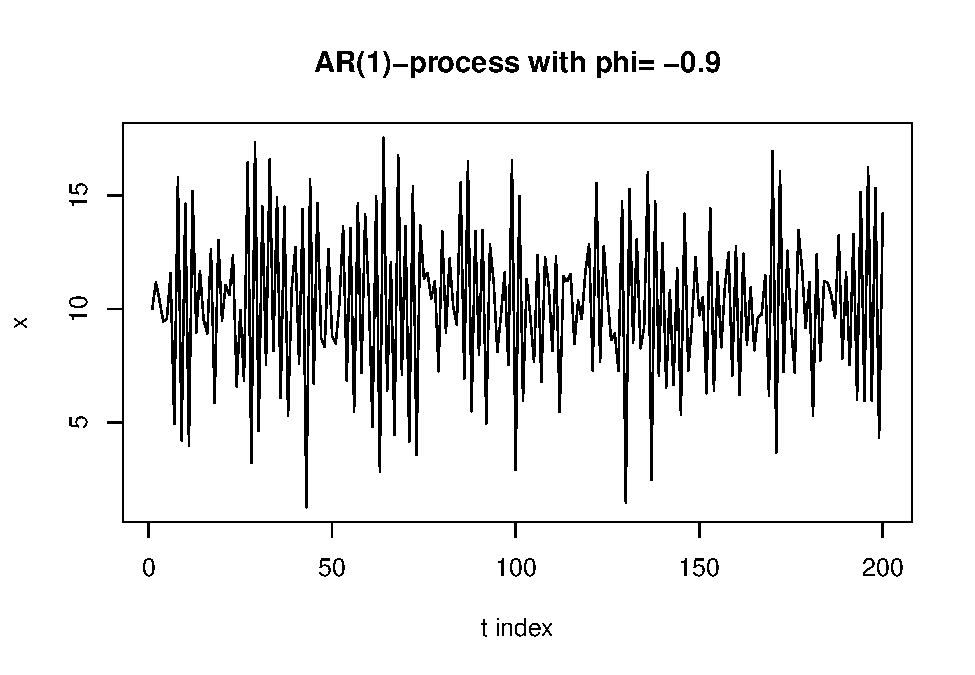
\includegraphics[width=0.8\linewidth]{lab3_mecon_files/figure-latex/unnamed-chunk-1-1} \end{center}

\begin{center}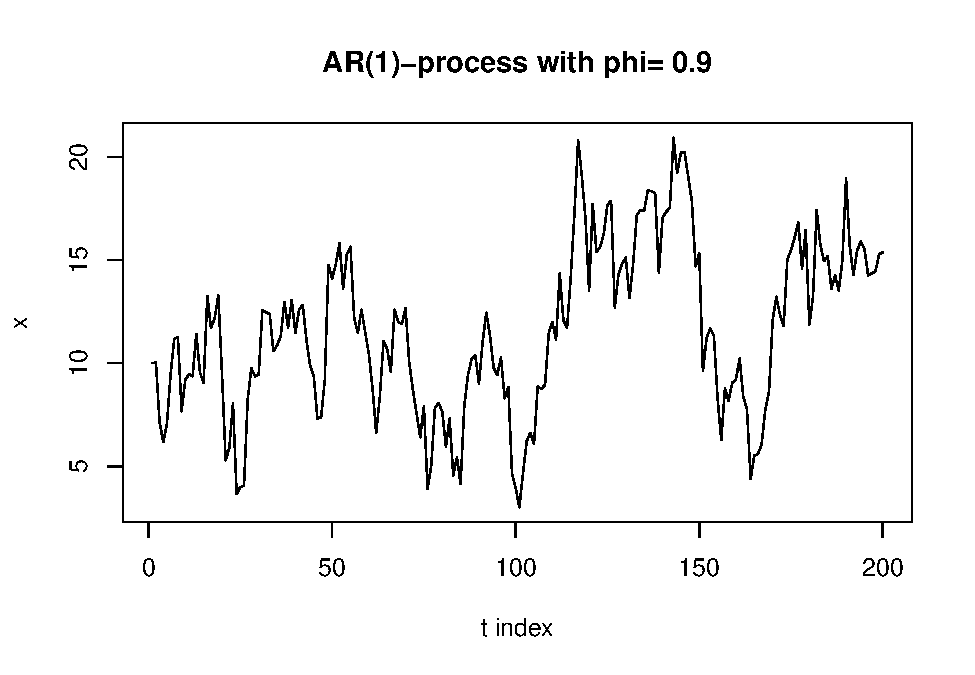
\includegraphics[width=0.8\linewidth]{lab3_mecon_files/figure-latex/unnamed-chunk-1-2} \end{center}

\hypertarget{ii.-analyze-the-daily-precipitation-using-your-gibbs-sampler-in-a-i.-evaluate-the-convergence-of-the-gibbs-sampler-by-suitable-graphical-methods-for-example-by-plotting-the-trajectories-of-the-sampled-markov-chains.}{%
\paragraph{ii. Analyze the daily precipitation using your Gibbs sampler
in (a)-i. Evaluate the convergence of the Gibbs sampler by suitable
graphical methods, for example by plotting the trajectories of the
sampled Markov
chains.}\label{ii.-analyze-the-daily-precipitation-using-your-gibbs-sampler-in-a-i.-evaluate-the-convergence-of-the-gibbs-sampler-by-suitable-graphical-methods-for-example-by-plotting-the-trajectories-of-the-sampled-markov-chains.}}

The below two graphs are shown the trajectory plot of the sampled Markov
chains. From the first graph of Posterior Variance trajectory, after
around 50 iterations burning period, it is towards converaged to the
true variance of the data which is about 1547.

From the second graph of Posterior Mean trajectory, the burning-period
of which is faster than the varanice, which within around 50 iterations.
After that, it is converaged to the true mean of the data which is about
32.28.

From the result, we can say that the Gibbs Sampling is a success, since
both Gibbs mean and variance are converaged to the true mean and
variance. Moreover, the burning period is fast and within 50 iterations,
based on the initiative parameters are set close to the given data.

\begin{center}\includegraphics[width=0.8\linewidth]{lab3_mecon_files/figure-latex/unnamed-chunk-2-1} \end{center}

\begin{center}\includegraphics[width=0.8\linewidth]{lab3_mecon_files/figure-latex/unnamed-chunk-2-2} \end{center}

\begin{verbatim}
## The value of Gibbs sampling of Mu: 32.29442
\end{verbatim}

\begin{verbatim}
## The value of Gibbs sampling of Sigma^2: 1546.928
\end{verbatim}

\hypertarget{b.-mixture-normal-model.}{%
\subsubsection{(b). Mixture normal
model.}\label{b.-mixture-normal-model.}}

Let us now instead assume that the daily precipitation
\({y_1 , ..., y_n}\) follow an iid two-component mixture of normals
model:
\[p(y_i|\mu,\sigma^2, \pi) = \pi N(y_i|\mu_1, \sigma_1^2) +(1-\pi)N(y_i|\mu_2,\sigma_2^2),\]
where

\[\mu = (\mu_1, \mu_2) \ \ and\ \ \sigma^2 = (\sigma_1^2, \sigma_2^2)\]

Use the Gibbs sampling data augmentation algorithm in
NormalMixtureGibbs.R (available under Lecture 7 on the course page) to
analyze the daily precipitation data. Set the prior hyperparameters
suitably. Evaluate the convergence of the sampler.

We set the same prior hyperparmeters as above. From 100 iterations, the
sampler converaged very fast from the first 20 iterations, and after
30th iterations the components do not change much. Therefore, we can say
in the algorithm of normal mixture, Gibbs sampling with the initial
hyperparameters work well in fitting the data.

\begin{center}\includegraphics[width=0.8\linewidth]{lab3_mecon_files/figure-latex/unnamed-chunk-3-1} \end{center}

\begin{center}\includegraphics[width=0.8\linewidth]{lab3_mecon_files/figure-latex/unnamed-chunk-3-2} \end{center}

\begin{center}\includegraphics[width=0.8\linewidth]{lab3_mecon_files/figure-latex/unnamed-chunk-3-3} \end{center}

\begin{center}\includegraphics[width=0.8\linewidth]{lab3_mecon_files/figure-latex/unnamed-chunk-3-4} \end{center}

\begin{center}\includegraphics[width=0.8\linewidth]{lab3_mecon_files/figure-latex/unnamed-chunk-3-5} \end{center}

\hypertarget{c-graphical-comparison.}{%
\subsubsection{(c) Graphical
comparison.}\label{c-graphical-comparison.}}

Plot the following densities in one figure: 1) a histogram or kernel
density estimate of the data. 2) Normal density
\(N(y_i |\mu, \sigma^2 )\) in (a); 3) Mixture of normals density
\(p(y_i |\mu, \sigma^2 , \pi)\) in (b). Base your plots on the mean over
all posterior draws.

Comparing with the Mixture of normal Density in (b) and Normal Density
from (a), we can easily spot that the Normal Density from (a) does not
fit well on the data density. However, using the mixture of normal
Density is fitted better than the nornal density one, though it is not
perfect, but still can cover most of the density of the original data.

\begin{center}\includegraphics[width=0.8\linewidth]{lab3_mecon_files/figure-latex/unnamed-chunk-4-1} \end{center}

\hypertarget{metropolis-random-walk-for-poisson-regression.}{%
\section{2. Metropolis Random Walk for Poisson
regression.}\label{metropolis-random-walk-for-poisson-regression.}}

Consider the following Poisson regression model
\[ y_i | \beta \sim Poisson[exp (x^T_i \beta)] , \ \ i = 1, ..., n,\]
where \(y_i\) is the count for the ith observation in the sample and
\(x_i\) is the p-dimensional vector with covariate observations for the
ith observation. Use the data set eBayNumberOfBidderData.dat. This
dataset contains observations from 1000 eBay auctions of coins. The
response variable is nBids and records the number of bids in each
auction. The remaining variables are features/covariates (x):

• Const (for the intercept) • PowerSeller (is the seller selling large
volumes on eBay?) • VerifyID (is the seller verified by eBay?) • Sealed
(was the coin sold sealed in never opened envelope?) • MinBlem (did the
coin have a minor defect?) • MajBlem (a major defect?) • LargNeg (did
the seller get a lot of negative feedback from customers?) • LogBook
(logarithm of the coins book value according to expert sellers.
Standardized) • MinBidShare (a variable that measures ratio of the
minimum selling price (starting price) to the book value. Standardized).

\hypertarget{a-obtain-the-maximum-likelihood-estimator-of-beta-in-the-poisson-regression-model-for-the-ebay-data-hint-glm.r-dont-forget-that-glm-adds-its-own-intercept-so-dont-input-the-covariate-const.-which-covariates-are-significant}{%
\subsubsection{\texorpdfstring{(a) Obtain the maximum likelihood
estimator of \(\beta\) in the Poisson regression model for the eBay data
{[}Hint: glm.R, don't forget that glm() adds its own intercept so don't
input the covariate Const{]}. Which covariates are
significant?}{(a) Obtain the maximum likelihood estimator of \textbackslash beta in the Poisson regression model for the eBay data {[}Hint: glm.R, don't forget that glm() adds its own intercept so don't input the covariate Const{]}. Which covariates are significant?}}\label{a-obtain-the-maximum-likelihood-estimator-of-beta-in-the-poisson-regression-model-for-the-ebay-data-hint-glm.r-dont-forget-that-glm-adds-its-own-intercept-so-dont-input-the-covariate-const.-which-covariates-are-significant}}

\begin{verbatim}
## The estimator of beta are: 1.072442 -0.02054076 -0.3945165 0.4438426 -0.05219829 -0.2208712 0.07067246 -0.1206776 -1.894097
\end{verbatim}

\begin{verbatim}
## 
## Call:
## glm(formula = nBids ~ ., family = "poisson", data = data1)
## 
## Deviance Residuals: 
##     Min       1Q   Median       3Q      Max  
## -3.5800  -0.7222  -0.0441   0.5269   2.4605  
## 
## Coefficients:
##             Estimate Std. Error z value Pr(>|z|)    
## (Intercept)  1.07244    0.03077  34.848  < 2e-16 ***
## PowerSeller -0.02054    0.03678  -0.558   0.5765    
## VerifyID    -0.39452    0.09243  -4.268 1.97e-05 ***
## Sealed       0.44384    0.05056   8.778  < 2e-16 ***
## Minblem     -0.05220    0.06020  -0.867   0.3859    
## MajBlem     -0.22087    0.09144  -2.416   0.0157 *  
## LargNeg      0.07067    0.05633   1.255   0.2096    
## LogBook     -0.12068    0.02896  -4.166 3.09e-05 ***
## MinBidShare -1.89410    0.07124 -26.588  < 2e-16 ***
## ---
## Signif. codes:  0 '***' 0.001 '**' 0.01 '*' 0.05 '.' 0.1 ' ' 1
## 
## (Dispersion parameter for poisson family taken to be 1)
## 
##     Null deviance: 2151.28  on 999  degrees of freedom
## Residual deviance:  867.47  on 991  degrees of freedom
## AIC: 3610.3
## 
## Number of Fisher Scoring iterations: 5
\end{verbatim}

By using glm() to obtain the summary of the Posisson regression model,
the most signficant covariates are having the most ***, which are
VerifyID, Sealed, LogBook and MinBidShare. BajBlem obtain only one star
so it is less significant. And the rest covariate are not influenced to
our model in this case.

From the significant covariates we can tell that, the most influenced
factor to the number of Bids is MinBidShare, the lower the selling price
is more appealing to bids.

\hypertarget{b-lets-now-do-a-bayesian-analysis-of-the-poisson-regression.-let-the-prior-be-beta-sim-n0100cdot-xt-x-1-where-x-is-the-n-x-p-covariate-matrix.-this-is-a-commonly-used-prior-which-is-called-zellners-g-prior.-assume-first-that-the-posterior-density-is-approximately-multivariate-normal}{%
\subsubsection{\texorpdfstring{(b) Let's now do a Bayesian analysis of
the Poisson regression. Let the prior be
\(\beta \sim N[0,100\cdot (X^T X)^(-1)]\) where X is the n x p covariate
matrix. This is a commonly used prior which is called Zellner's g-prior.
Assume first that the posterior density is approximately multivariate
normal:}{(b) Let's now do a Bayesian analysis of the Poisson regression. Let the prior be \textbackslash beta \textbackslash sim N{[}0,100\textbackslash cdot (X\^{}T X)\^{}(-1){]} where X is the n x p covariate matrix. This is a commonly used prior which is called Zellner's g-prior. Assume first that the posterior density is approximately multivariate normal:}}\label{b-lets-now-do-a-bayesian-analysis-of-the-poisson-regression.-let-the-prior-be-beta-sim-n0100cdot-xt-x-1-where-x-is-the-n-x-p-covariate-matrix.-this-is-a-commonly-used-prior-which-is-called-zellners-g-prior.-assume-first-that-the-posterior-density-is-approximately-multivariate-normal}}

\[ \beta|y \sim N( \widetilde{\beta}, J^{-1}_y (\tilde{\beta})) \]

\hypertarget{where-tildebeta-is-the-posterior-mode-and-j_ytildebeta-is-the-negative-hessian-at-the-posterior-mode.-tildebeta-and-j_ytildebeta-can-be-obtained-by-numerical-optimization-optim.r-exactly-like-you-already-did-for-the-logistic-regression-in-lab-2-but-with-the-log-posterior-function-replaced-by-the-corresponding-one-for-the-poisson-model-which-you-have-to-code-up}{%
\subsubsection{\texorpdfstring{where \(\tilde{\beta}\) is the posterior
mode and \(J_y(\tilde{\beta})\) is the negative Hessian at the posterior
mode. \(\tilde{\beta}\) and \(J_y(\tilde{\beta})\) can be obtained by
numerical optimization (optim.R) exactly like you already did for the
logistic regression in Lab 2 (but with the log posterior function
replaced by the corresponding one for the Poisson model, which you have
to code
up)}{where \textbackslash tilde\{\textbackslash beta\} is the posterior mode and J\_y(\textbackslash tilde\{\textbackslash beta\}) is the negative Hessian at the posterior mode. \textbackslash tilde\{\textbackslash beta\} and J\_y(\textbackslash tilde\{\textbackslash beta\}) can be obtained by numerical optimization (optim.R) exactly like you already did for the logistic regression in Lab 2 (but with the log posterior function replaced by the corresponding one for the Poisson model, which you have to code up)}}\label{where-tildebeta-is-the-posterior-mode-and-j_ytildebeta-is-the-negative-hessian-at-the-posterior-mode.-tildebeta-and-j_ytildebeta-can-be-obtained-by-numerical-optimization-optim.r-exactly-like-you-already-did-for-the-logistic-regression-in-lab-2-but-with-the-log-posterior-function-replaced-by-the-corresponding-one-for-the-poisson-model-which-you-have-to-code-up}}

\emph{Likelihood of Poisson Regression}
\[p(y|X,\tilde{\beta}) = \prod^n_{i=1} \frac{exp(y_i \tilde{\beta}x_i)-exp(-exp(\tilde{\beta x_i}))}{y_i!}\]

\emph{Log-likelihood of poisson regression}
\[p(y_i|x_i,\tilde{\beta}) = \sum^n_{i=1}(y_i\tilde{\beta}x_i -exp(\tilde{\beta}x_i)-log(y_i!)) \]

\begin{longtable}[]{@{}lrrrrrrrrr@{}}
\toprule
& Const & PowerSeller & VerifyID & Sealed & Minblem & MajBlem & LargNeg
& LogBook & MinBidShare\tabularnewline
\midrule
\endhead
Const & 0.0009455 & -0.0007139 & -0.0002742 & -0.0002709 & -0.0004455 &
-0.0002772 & -0.0005128 & 0.0000644 & 0.0011099\tabularnewline
PowerSeller & -0.0007139 & 0.0013531 & 0.0000402 & -0.0002949 &
0.0001143 & -0.0002083 & 0.0002802 & 0.0001182 &
-0.0005686\tabularnewline
VerifyID & -0.0002742 & 0.0000402 & 0.0085154 & -0.0007825 & -0.0001014
& 0.0002283 & 0.0003314 & -0.0003192 & -0.0004293\tabularnewline
Sealed & -0.0002709 & -0.0002949 & -0.0007825 & 0.0025578 & 0.0003577 &
0.0004532 & 0.0003376 & -0.0001311 & -0.0000576\tabularnewline
Minblem & -0.0004455 & 0.0001143 & -0.0001014 & 0.0003577 & 0.0036246 &
0.0003492 & 0.0000584 & 0.0000585 & -0.0000644\tabularnewline
MajBlem & -0.0002772 & -0.0002083 & 0.0002283 & 0.0004532 & 0.0003492 &
0.0083651 & 0.0004049 & -0.0000898 & 0.0002622\tabularnewline
LargNeg & -0.0005128 & 0.0002802 & 0.0003314 & 0.0003376 & 0.0000584 &
0.0004049 & 0.0031751 & -0.0002542 & -0.0001063\tabularnewline
LogBook & 0.0000644 & 0.0001182 & -0.0003192 & -0.0001311 & 0.0000585 &
-0.0000898 & -0.0002542 & 0.0008385 & 0.0010374\tabularnewline
MinBidShare & 0.0011099 & -0.0005686 & -0.0004293 & -0.0000576 &
-0.0000644 & 0.0002622 & -0.0001063 & 0.0010374 &
0.0050548\tabularnewline
\bottomrule
\end{longtable}

\begin{longtable}[]{@{}lr@{}}
\toprule
& Approximate Beta tilde\tabularnewline
\midrule
\endhead
Const & 1.0698412\tabularnewline
PowerSeller & -0.0205125\tabularnewline
VerifyID & -0.3930060\tabularnewline
Sealed & 0.4435555\tabularnewline
Minblem & -0.0524663\tabularnewline
MajBlem & -0.2212384\tabularnewline
LargNeg & 0.0706968\tabularnewline
LogBook & -0.1202177\tabularnewline
MinBidShare & -1.8919850\tabularnewline
\bottomrule
\end{longtable}

Comparing to the maximum likelihood estimator \(\beta\) we obtained in
(a), the posterior mode \(\tilde{\beta}\) the result obtained by
numerical optimization is very close to \(\beta\).

\hypertarget{c-now-lets-simulate-from-the-actual-posterior-of-beta-using-the-metropolis-algorithm-and-compare-with-the-approximate-results-in-b.-program-a-general-function-that-uses-the-metropolis-algorithm-to-generate-random-draws-from-an-arbitrary-posterior-density.-in-order-to-show-that-it-is-a-general-function-for-any-model-i-will-denote-the-vector-of-model-parameters-by-theta.-let-the-proposal-density-be-the-multivariate-normal-density-mentioned-in-lecture-8-random-walk-metropolis}{%
\subsubsection{\texorpdfstring{(c) Now, let's simulate from the actual
posterior of \(\beta\) using the Metropolis algorithm and compare with
the approximate results in b). Program a general function that uses the
Metropolis algorithm to generate random draws from an arbitrary
posterior density. In order to show that it is a general function for
any model, I will denote the vector of model parameters by \(\theta\).
Let the proposal density be the multivariate normal density mentioned in
Lecture 8 (random walk
Metropolis):}{(c) Now, let's simulate from the actual posterior of \textbackslash beta using the Metropolis algorithm and compare with the approximate results in b). Program a general function that uses the Metropolis algorithm to generate random draws from an arbitrary posterior density. In order to show that it is a general function for any model, I will denote the vector of model parameters by \textbackslash theta. Let the proposal density be the multivariate normal density mentioned in Lecture 8 (random walk Metropolis):}}\label{c-now-lets-simulate-from-the-actual-posterior-of-beta-using-the-metropolis-algorithm-and-compare-with-the-approximate-results-in-b.-program-a-general-function-that-uses-the-metropolis-algorithm-to-generate-random-draws-from-an-arbitrary-posterior-density.-in-order-to-show-that-it-is-a-general-function-for-any-model-i-will-denote-the-vector-of-model-parameters-by-theta.-let-the-proposal-density-be-the-multivariate-normal-density-mentioned-in-lecture-8-random-walk-metropolis}}

\[\theta_p | \theta^{i−1} \sim N(\theta^{i−1}, c \cdot \Sigma) ,\] where
\(\Sigma = J^{-1}_y(\tilde{\beta})\)

\begin{center}\includegraphics[width=0.8\linewidth]{lab3_mecon_files/figure-latex/unnamed-chunk-7-1} \end{center}

\hypertarget{d-use-the-mcmc-draws-from-c-to-simulate-from-the-predictive-distribution-of-the-number-of-bidders-in-a-new-auction-with-the-characteristics-below.-plot-the-predictive-distribution.-what-is-the-probability-of-no-bidders-in-this-new-auction}{%
\subsubsection{(d) Use the MCMC draws from c) to simulate from the
predictive distribution of the number of bidders in a new auction with
the characteristics below. Plot the predictive distribution. What is the
probability of no bidders in this new
auction?}\label{d-use-the-mcmc-draws-from-c-to-simulate-from-the-predictive-distribution-of-the-number-of-bidders-in-a-new-auction-with-the-characteristics-below.-plot-the-predictive-distribution.-what-is-the-probability-of-no-bidders-in-this-new-auction}}

• PowerSeller = 1 • VerifyID = 1 • Sealed = 1 • MinBlem = 0 • MajBlem =
0 • LargNeg = 0 • LogBook = 1 • MinBidShare = 0.5

\hypertarget{appendix}{%
\section{Appendix}\label{appendix}}

\begin{Shaded}
\begin{Highlighting}[]
\KeywordTok{library}\NormalTok{(LaplacesDemon)}
\CommentTok{\# 1.}
\CommentTok{\#\# (a)}
\CommentTok{\#\#\#.i. Gibbs sampler from joint posterior}
\NormalTok{data =}\StringTok{ }\KeywordTok{read.table}\NormalTok{(}\StringTok{"rainfall.dat"}\NormalTok{)}

\CommentTok{\# para from data}
\NormalTok{n =}\StringTok{ }\KeywordTok{length}\NormalTok{(}\KeywordTok{row}\NormalTok{(data)) }\CommentTok{\#6920}
\NormalTok{xbar =}\StringTok{ }\KeywordTok{mean}\NormalTok{(data}\OperatorTok{$}\NormalTok{V1) }\CommentTok{\#32.28}
\KeywordTok{var}\NormalTok{(data}\OperatorTok{$}\NormalTok{V1)}

\CommentTok{\#set up parameters}
\NormalTok{mu0 =}\StringTok{ }\DecValTok{30} \CommentTok{\#True mean =32.28 }
\NormalTok{tau20 =}\StringTok{ }\DecValTok{150} \CommentTok{\# we dont have prior knowledge}
\NormalTok{nu0 =}\StringTok{ }\DecValTok{3} \CommentTok{\#df set it to a small value}
\NormalTok{sigma20 =}\StringTok{ }\KeywordTok{var}\NormalTok{(data}\OperatorTok{$}\NormalTok{V1) }\CommentTok{\#True var=1547.103}

\CommentTok{\#\# Gibbs sampling}
\NormalTok{Ndraws =}\StringTok{ }\DecValTok{1000}
\NormalTok{GibbMu =}\StringTok{ }\KeywordTok{c}\NormalTok{()}
\NormalTok{GibbMu[}\DecValTok{1}\NormalTok{] =}\StringTok{ }\NormalTok{mu0}
\NormalTok{GibbSigma2 =}\StringTok{ }\KeywordTok{c}\NormalTok{()}
\NormalTok{GibbSigma2[}\DecValTok{1}\NormalTok{] =}\StringTok{ }\NormalTok{sigma20}

\KeywordTok{set.seed}\NormalTok{(}\DecValTok{12345}\NormalTok{)}
\ControlFlowTok{for}\NormalTok{(i }\ControlFlowTok{in} \DecValTok{1}\OperatorTok{:}\NormalTok{Ndraws)\{}
  \CommentTok{\# parameters w mu tau, update mu\_n, tau\_n}
\NormalTok{  w =}\StringTok{ }\NormalTok{(n}\OperatorTok{/}\NormalTok{GibbSigma2[i]) }\OperatorTok{/}\StringTok{ }\NormalTok{( (n}\OperatorTok{/}\NormalTok{GibbSigma2) }\OperatorTok{+}\StringTok{ }\NormalTok{(}\DecValTok{1}\OperatorTok{/}\NormalTok{tau20) )}
\NormalTok{  mu\_n =}\StringTok{ }\NormalTok{w}\OperatorTok{*}\NormalTok{xbar }\OperatorTok{+}\StringTok{ }\NormalTok{(}\DecValTok{1}\OperatorTok{{-}}\NormalTok{w)}\OperatorTok{*}\NormalTok{mu0}
\NormalTok{  tau\_n =}\StringTok{ }\DecValTok{1}\OperatorTok{/}\StringTok{ }\NormalTok{( (n}\OperatorTok{/}\NormalTok{GibbSigma2[i]) }\OperatorTok{+}\StringTok{ }\NormalTok{(}\DecValTok{1}\OperatorTok{/}\NormalTok{tau20)  )}
  
  \CommentTok{\# sampling posterior mu, add in mu}
\NormalTok{  GibbMu[i}\OperatorTok{+}\DecValTok{1}\NormalTok{] =}\StringTok{ }\KeywordTok{rnorm}\NormalTok{(}\DecValTok{1}\NormalTok{, }\DataTypeTok{mean=}\NormalTok{mu\_n, }\DataTypeTok{sd=}\NormalTok{tau\_n)}
  
  \CommentTok{\#sampling posterior sigma2, add in sigma2}
\NormalTok{  nu\_n =}\StringTok{ }\NormalTok{nu0 }\OperatorTok{+}\StringTok{ }\NormalTok{n}
\NormalTok{  Scale =(nu0}\OperatorTok{*}\NormalTok{sigma20 }\OperatorTok{+}\StringTok{ }\KeywordTok{sum}\NormalTok{((data}\OperatorTok{$}\NormalTok{V1 }\OperatorTok{{-}}\StringTok{ }\NormalTok{GibbMu[i}\OperatorTok{+}\DecValTok{1}\NormalTok{])}\OperatorTok{\^{}}\DecValTok{2}\NormalTok{) )}\OperatorTok{/}\StringTok{ }\NormalTok{(n}\OperatorTok{+}\NormalTok{nu0)}
\NormalTok{  GibbSigma2[i}\OperatorTok{+}\DecValTok{1}\NormalTok{] =}\StringTok{ }\KeywordTok{rinvchisq}\NormalTok{(}\DecValTok{1}\NormalTok{, }\DataTypeTok{df=}\NormalTok{ nu\_n, }\DataTypeTok{scale=}\NormalTok{ Scale)}
\NormalTok{\}}

\KeywordTok{hist}\NormalTok{(GibbSigma2,}\DataTypeTok{breaks=}\DecValTok{20}\NormalTok{, }\DataTypeTok{main=}\StringTok{"Histogram of Gibbs samplers of sigma\^{}2"}\NormalTok{, }\DataTypeTok{xlab=}\StringTok{"Gibbs samplers of sigma\^{}2"}\NormalTok{)}
\KeywordTok{hist}\NormalTok{(GibbMu, }\DataTypeTok{breaks=}\DecValTok{30}\NormalTok{, }\DataTypeTok{main=}\StringTok{"Histogram of Gibbs samplers of Mu"}\NormalTok{, }\DataTypeTok{xlab=}\StringTok{"Gibbs samplers of mu"}\NormalTok{)}


\CommentTok{\#\#\# ii. }
\NormalTok{cumMu=}\KeywordTok{c}\NormalTok{()}
\NormalTok{cumSigma2=}\KeywordTok{c}\NormalTok{()}

\CommentTok{\# plot variance MC converage}
\KeywordTok{plot}\NormalTok{(GibbSigma2, }\DataTypeTok{type=}\StringTok{"l"}\NormalTok{,}\DataTypeTok{col=}\StringTok{"darkgrey"}\NormalTok{, }\DataTypeTok{main=}\StringTok{"Posterior Variance trjectory"}\NormalTok{, }\DataTypeTok{xlab=}\StringTok{"Iteration"}\NormalTok{,}\DataTypeTok{ylab=}\StringTok{"Gibb sample of Variance"}\NormalTok{)}
\KeywordTok{abline}\NormalTok{(}\DataTypeTok{h=}\KeywordTok{var}\NormalTok{(data}\OperatorTok{$}\NormalTok{V1), }\DataTypeTok{col=}\StringTok{"green"}\NormalTok{, }\DataTypeTok{lwd=}\DecValTok{2}\NormalTok{)}
\KeywordTok{legend}\NormalTok{(}\StringTok{"bottomright"}\NormalTok{,}\DataTypeTok{legend=}\KeywordTok{c}\NormalTok{(}\StringTok{"Cumulative Mean"}\NormalTok{, }\StringTok{"True"}\NormalTok{), }\DataTypeTok{col=}\KeywordTok{c}\NormalTok{(}\StringTok{"red"}\NormalTok{,}\StringTok{"green"}\NormalTok{),}\DataTypeTok{lwd=}\DecValTok{2}\NormalTok{)}
\ControlFlowTok{for}\NormalTok{(i }\ControlFlowTok{in} \DecValTok{1}\OperatorTok{:}\KeywordTok{length}\NormalTok{(GibbSigma2))\{}
\NormalTok{  cumSigma2[i] =}\StringTok{ }\KeywordTok{mean}\NormalTok{(GibbSigma2[}\DecValTok{1}\OperatorTok{:}\NormalTok{i])}
  \KeywordTok{lines}\NormalTok{(cumSigma2, }\DataTypeTok{col=}\StringTok{"red"}\NormalTok{, }\DataTypeTok{lwd=}\DecValTok{2}\NormalTok{)}
\NormalTok{\}}

\CommentTok{\# plot mean MC converage}
\KeywordTok{plot}\NormalTok{(GibbMu, }\DataTypeTok{type=}\StringTok{"l"}\NormalTok{, }\DataTypeTok{col=}\StringTok{"darkgrey"}\NormalTok{, }\DataTypeTok{main=}\StringTok{"Posterior Mean trajectory"}\NormalTok{, }\DataTypeTok{xlab=}\StringTok{"Iteration"}\NormalTok{, }\DataTypeTok{ylab=}\StringTok{"Gibb sample of Mean"}\NormalTok{ )}
\KeywordTok{abline}\NormalTok{(}\DataTypeTok{h=}\NormalTok{xbar, }\DataTypeTok{col=}\StringTok{"green"}\NormalTok{, }\DataTypeTok{lwd=}\DecValTok{2}\NormalTok{)}
\KeywordTok{legend}\NormalTok{(}\StringTok{"bottomright"}\NormalTok{,}\DataTypeTok{legend=}\KeywordTok{c}\NormalTok{(}\StringTok{"Cumulative Mean"}\NormalTok{, }\StringTok{"True"}\NormalTok{), }\DataTypeTok{col=}\KeywordTok{c}\NormalTok{(}\StringTok{"red"}\NormalTok{,}\StringTok{"green"}\NormalTok{),}\DataTypeTok{lwd=}\DecValTok{2}\NormalTok{)}
\ControlFlowTok{for}\NormalTok{(i }\ControlFlowTok{in} \DecValTok{1}\OperatorTok{:}\KeywordTok{length}\NormalTok{(GibbMu))\{}
\NormalTok{  cumMu[i]=}\StringTok{ }\KeywordTok{mean}\NormalTok{(GibbMu[}\DecValTok{1}\OperatorTok{:}\NormalTok{i])}
  \KeywordTok{lines}\NormalTok{(cumMu,}\DataTypeTok{col=}\StringTok{"red"}\NormalTok{, }\DataTypeTok{lwd=}\DecValTok{2}\NormalTok{)}
\NormalTok{\}}
\KeywordTok{cat}\NormalTok{(}\StringTok{"The value of Gibbs sampling of Mu:"}\NormalTok{,}\KeywordTok{mean}\NormalTok{(GibbMu))}
\KeywordTok{cat}\NormalTok{(}\StringTok{"The value of Gibbs sampling of Sigma\^{}2:"}\NormalTok{, }\KeywordTok{mean}\NormalTok{(GibbSigma2))}


\CommentTok{\# 1.b}

\CommentTok{\# Estimating a simple mixture of normals}
\CommentTok{\# Author: Mattias Villani, IDA, Linkoping University. http://mattiasvillani.com}

\CommentTok{\#\#\#\#\#\#\#\#\#\#    }\RegionMarkerTok{BEGIN}\CommentTok{ USER INPUT \#\#\#\#\#\#\#\#\#\#\#\#\#\#\#\#\#}
\CommentTok{\# Data options}
\CommentTok{\#data(faithful)}
\CommentTok{\#rawData \textless{}{-} faithful}
\NormalTok{x \textless{}{-}}\StringTok{ }\KeywordTok{as.matrix}\NormalTok{(data}\OperatorTok{$}\NormalTok{V1)}

\CommentTok{\# Model options}
\NormalTok{nComp \textless{}{-}}\StringTok{ }\DecValTok{2}    \CommentTok{\# Number of mixture components}

\CommentTok{\# Prior options}
\NormalTok{alpha \textless{}{-}}\StringTok{ }\DecValTok{10}\OperatorTok{*}\KeywordTok{rep}\NormalTok{(}\DecValTok{1}\NormalTok{,nComp) }\CommentTok{\# Dirichlet(alpha)}
\NormalTok{muPrior \textless{}{-}}\StringTok{ }\KeywordTok{rep}\NormalTok{(}\DecValTok{30}\NormalTok{,nComp) }\CommentTok{\# Prior mean of mu}
\NormalTok{tau2Prior \textless{}{-}}\StringTok{ }\KeywordTok{rep}\NormalTok{(}\DecValTok{150}\NormalTok{,nComp) }\CommentTok{\# Prior std of mu}
\NormalTok{sigma2\_}\DecValTok{0}\NormalTok{ \textless{}{-}}\StringTok{ }\KeywordTok{rep}\NormalTok{(}\KeywordTok{var}\NormalTok{(x),nComp) }\CommentTok{\# s20 (best guess of sigma2)}
\NormalTok{nu0 \textless{}{-}}\StringTok{ }\KeywordTok{rep}\NormalTok{(}\DecValTok{3}\NormalTok{,nComp) }\CommentTok{\# degrees of freedom for prior on sigma2}

\CommentTok{\# MCMC options}
\NormalTok{nIter \textless{}{-}}\StringTok{ }\DecValTok{100} \CommentTok{\# Number of Gibbs sampling draws}

\CommentTok{\# Plotting options}
\NormalTok{plotFit \textless{}{-}}\StringTok{ }\OtherTok{TRUE}
\NormalTok{lineColors \textless{}{-}}\StringTok{ }\KeywordTok{c}\NormalTok{(}\StringTok{"blue"}\NormalTok{, }\StringTok{"green"}\NormalTok{, }\StringTok{"magenta"}\NormalTok{, }\StringTok{\textquotesingle{}yellow\textquotesingle{}}\NormalTok{)}
\CommentTok{\#sleepTime \textless{}{-} 0.1 \# Adding sleep time between iterations for plotting}
\CommentTok{\#\#\#\#\#\#\#\#\#\#\#\#\#\#\#\#   }\RegionMarkerTok{END}\CommentTok{ USER INPUT \#\#\#\#\#\#\#\#\#\#\#\#\#\#\#}

\CommentTok{\#\#\#\#\#\# Defining a function that simulates from the }
\NormalTok{rScaledInvChi2 \textless{}{-}}\StringTok{ }\ControlFlowTok{function}\NormalTok{(n, df, scale)\{}
  \KeywordTok{return}\NormalTok{((df}\OperatorTok{*}\NormalTok{scale)}\OperatorTok{/}\KeywordTok{rchisq}\NormalTok{(n,}\DataTypeTok{df=}\NormalTok{df))}
\NormalTok{\}}

\CommentTok{\#\#\#\#\#\#\# Defining a function that simulates from a Dirichlet distribution}
\NormalTok{rDirichlet \textless{}{-}}\StringTok{ }\ControlFlowTok{function}\NormalTok{(param)\{}
\NormalTok{  nCat \textless{}{-}}\StringTok{ }\KeywordTok{length}\NormalTok{(param)}
\NormalTok{  piDraws \textless{}{-}}\StringTok{ }\KeywordTok{matrix}\NormalTok{(}\OtherTok{NA}\NormalTok{,nCat,}\DecValTok{1}\NormalTok{)}
  \ControlFlowTok{for}\NormalTok{ (j }\ControlFlowTok{in} \DecValTok{1}\OperatorTok{:}\NormalTok{nCat)\{}
\NormalTok{    piDraws[j] \textless{}{-}}\StringTok{ }\KeywordTok{rgamma}\NormalTok{(}\DecValTok{1}\NormalTok{,param[j],}\DecValTok{1}\NormalTok{)}
\NormalTok{  \}}
\NormalTok{  piDraws =}\StringTok{ }\NormalTok{piDraws}\OperatorTok{/}\KeywordTok{sum}\NormalTok{(piDraws) }\CommentTok{\# Diving every column of piDraws by the sum of the elements in that column.}
  \KeywordTok{return}\NormalTok{(piDraws)}
\NormalTok{\}}

\CommentTok{\# Simple function that converts between two different representations of the mixture allocation}
\NormalTok{S2alloc \textless{}{-}}\StringTok{ }\ControlFlowTok{function}\NormalTok{(S)\{}
\NormalTok{  n \textless{}{-}}\StringTok{ }\KeywordTok{dim}\NormalTok{(S)[}\DecValTok{1}\NormalTok{]}
\NormalTok{  alloc \textless{}{-}}\StringTok{ }\KeywordTok{rep}\NormalTok{(}\DecValTok{0}\NormalTok{,n)}
  \ControlFlowTok{for}\NormalTok{ (i }\ControlFlowTok{in} \DecValTok{1}\OperatorTok{:}\NormalTok{n)\{}
\NormalTok{    alloc[i] \textless{}{-}}\StringTok{ }\KeywordTok{which}\NormalTok{(S[i,] }\OperatorTok{==}\StringTok{ }\DecValTok{1}\NormalTok{)}
\NormalTok{  \}}
  \KeywordTok{return}\NormalTok{(alloc)}
\NormalTok{\}}

\CommentTok{\# Initial value for the MCMC}
\NormalTok{nObs \textless{}{-}}\StringTok{ }\KeywordTok{length}\NormalTok{(x)}
\NormalTok{S \textless{}{-}}\StringTok{ }\KeywordTok{t}\NormalTok{(}\KeywordTok{rmultinom}\NormalTok{(nObs, }\DataTypeTok{size =} \DecValTok{1}\NormalTok{ , }\DataTypeTok{prob =} \KeywordTok{rep}\NormalTok{(}\DecValTok{1}\OperatorTok{/}\NormalTok{nComp,nComp))) }\CommentTok{\# nObs{-}by{-}nComp matrix with component allocations.}
\NormalTok{mu \textless{}{-}}\StringTok{ }\KeywordTok{quantile}\NormalTok{(x, }\DataTypeTok{probs =} \KeywordTok{seq}\NormalTok{(}\DecValTok{0}\NormalTok{,}\DecValTok{1}\NormalTok{,}\DataTypeTok{length =}\NormalTok{ nComp))}
\NormalTok{sigma2 \textless{}{-}}\StringTok{ }\KeywordTok{rep}\NormalTok{(}\KeywordTok{var}\NormalTok{(x),nComp)}
\NormalTok{probObsInComp \textless{}{-}}\StringTok{ }\KeywordTok{rep}\NormalTok{(}\OtherTok{NA}\NormalTok{, nComp)}

\CommentTok{\# Setting up the plot}
\NormalTok{xGrid \textless{}{-}}\StringTok{ }\KeywordTok{seq}\NormalTok{(}\KeywordTok{min}\NormalTok{(x)}\OperatorTok{{-}}\DecValTok{1}\OperatorTok{*}\KeywordTok{apply}\NormalTok{(x,}\DecValTok{2}\NormalTok{,sd),}\KeywordTok{max}\NormalTok{(x)}\OperatorTok{+}\DecValTok{1}\OperatorTok{*}\KeywordTok{apply}\NormalTok{(x,}\DecValTok{2}\NormalTok{,sd),}\DataTypeTok{length =} \DecValTok{100}\NormalTok{)}
\NormalTok{xGridMin \textless{}{-}}\StringTok{ }\KeywordTok{min}\NormalTok{(xGrid)}
\NormalTok{xGridMax \textless{}{-}}\StringTok{ }\KeywordTok{max}\NormalTok{(xGrid)}
\NormalTok{mixDensMean \textless{}{-}}\StringTok{ }\KeywordTok{rep}\NormalTok{(}\DecValTok{0}\NormalTok{,}\KeywordTok{length}\NormalTok{(xGrid))}
\NormalTok{effIterCount \textless{}{-}}\StringTok{ }\DecValTok{0}
\NormalTok{ylim \textless{}{-}}\StringTok{ }\KeywordTok{c}\NormalTok{(}\DecValTok{0}\NormalTok{,}\DecValTok{2}\OperatorTok{*}\KeywordTok{max}\NormalTok{(}\KeywordTok{hist}\NormalTok{(x)}\OperatorTok{$}\NormalTok{density))}


\ControlFlowTok{for}\NormalTok{ (k }\ControlFlowTok{in} \DecValTok{1}\OperatorTok{:}\NormalTok{nIter)\{}
  \CommentTok{\#message(paste(\textquotesingle{}Iteration number:\textquotesingle{},k))}
\NormalTok{  alloc \textless{}{-}}\StringTok{ }\KeywordTok{S2alloc}\NormalTok{(S) }\CommentTok{\# Just a function that converts between different representations of the group allocations}
\NormalTok{  nAlloc \textless{}{-}}\StringTok{ }\KeywordTok{colSums}\NormalTok{(S)}
  \CommentTok{\#print(nAlloc)}
  \CommentTok{\# Update components probabilities}
\NormalTok{  pi \textless{}{-}}\StringTok{ }\KeywordTok{rDirichlet}\NormalTok{(alpha }\OperatorTok{+}\StringTok{ }\NormalTok{nAlloc)}
  
  \CommentTok{\# Update mu\textquotesingle{}s}
  \ControlFlowTok{for}\NormalTok{ (j }\ControlFlowTok{in} \DecValTok{1}\OperatorTok{:}\NormalTok{nComp)\{}
\NormalTok{    precPrior \textless{}{-}}\StringTok{ }\DecValTok{1}\OperatorTok{/}\NormalTok{tau2Prior[j]}
\NormalTok{    precData \textless{}{-}}\StringTok{ }\NormalTok{nAlloc[j]}\OperatorTok{/}\NormalTok{sigma2[j]}
\NormalTok{    precPost \textless{}{-}}\StringTok{ }\NormalTok{precPrior }\OperatorTok{+}\StringTok{ }\NormalTok{precData}
\NormalTok{    wPrior \textless{}{-}}\StringTok{ }\NormalTok{precPrior}\OperatorTok{/}\NormalTok{precPost}
\NormalTok{    muPost \textless{}{-}}\StringTok{ }\NormalTok{wPrior}\OperatorTok{*}\NormalTok{muPrior }\OperatorTok{+}\StringTok{ }\NormalTok{(}\DecValTok{1}\OperatorTok{{-}}\NormalTok{wPrior)}\OperatorTok{*}\KeywordTok{mean}\NormalTok{(x[alloc }\OperatorTok{==}\StringTok{ }\NormalTok{j])}
\NormalTok{    tau2Post \textless{}{-}}\StringTok{ }\DecValTok{1}\OperatorTok{/}\NormalTok{precPost}
\NormalTok{    mu[j] \textless{}{-}}\StringTok{ }\KeywordTok{rnorm}\NormalTok{(}\DecValTok{1}\NormalTok{, }\DataTypeTok{mean =}\NormalTok{ muPost, }\DataTypeTok{sd =} \KeywordTok{sqrt}\NormalTok{(tau2Post))}
\NormalTok{  \}}
  
  \CommentTok{\# Update sigma2\textquotesingle{}s}
  \ControlFlowTok{for}\NormalTok{ (j }\ControlFlowTok{in} \DecValTok{1}\OperatorTok{:}\NormalTok{nComp)\{}
\NormalTok{    sigma2[j] \textless{}{-}}\StringTok{ }\KeywordTok{rScaledInvChi2}\NormalTok{(}\DecValTok{1}\NormalTok{, }\DataTypeTok{df =}\NormalTok{ nu0[j] }\OperatorTok{+}\StringTok{ }\NormalTok{nAlloc[j], }\DataTypeTok{scale =}\NormalTok{ (nu0[j]}\OperatorTok{*}\NormalTok{sigma2\_}\DecValTok{0}\NormalTok{[j] }\OperatorTok{+}\StringTok{ }\KeywordTok{sum}\NormalTok{((x[alloc }\OperatorTok{==}\StringTok{ }\NormalTok{j] }\OperatorTok{{-}}\StringTok{ }\NormalTok{mu[j])}\OperatorTok{\^{}}\DecValTok{2}\NormalTok{))}\OperatorTok{/}\NormalTok{(nu0[j] }\OperatorTok{+}\StringTok{ }\NormalTok{nAlloc[j]))}
\NormalTok{  \}}
  
  \CommentTok{\# Update allocation}
  \ControlFlowTok{for}\NormalTok{ (i }\ControlFlowTok{in} \DecValTok{1}\OperatorTok{:}\NormalTok{nObs)\{}
    \ControlFlowTok{for}\NormalTok{ (j }\ControlFlowTok{in} \DecValTok{1}\OperatorTok{:}\NormalTok{nComp)\{}
\NormalTok{      probObsInComp[j] \textless{}{-}}\StringTok{ }\NormalTok{pi[j]}\OperatorTok{*}\KeywordTok{dnorm}\NormalTok{(x[i], }\DataTypeTok{mean =}\NormalTok{ mu[j], }\DataTypeTok{sd =} \KeywordTok{sqrt}\NormalTok{(sigma2[j]))}
\NormalTok{    \}}
\NormalTok{    S[i,] \textless{}{-}}\StringTok{ }\KeywordTok{t}\NormalTok{(}\KeywordTok{rmultinom}\NormalTok{(}\DecValTok{1}\NormalTok{, }\DataTypeTok{size =} \DecValTok{1}\NormalTok{ , }\DataTypeTok{prob =}\NormalTok{ probObsInComp}\OperatorTok{/}\KeywordTok{sum}\NormalTok{(probObsInComp)))}
\NormalTok{  \}}
  
  
  \CommentTok{\# Printing the fitted density against data histogram}
  \ControlFlowTok{if}\NormalTok{(k }\OperatorTok{\%in\%}\StringTok{ }\KeywordTok{c}\NormalTok{(}\DecValTok{10}\NormalTok{,}\DecValTok{30}\NormalTok{,}\DecValTok{50}\NormalTok{,}\DecValTok{100}\NormalTok{) )\{}
  \ControlFlowTok{if}\NormalTok{ (plotFit }\OperatorTok{\&\&}\StringTok{ }\NormalTok{(k}\OperatorTok{\%\%}\DecValTok{1} \OperatorTok{==}\DecValTok{0}\NormalTok{))\{}
\NormalTok{    effIterCount \textless{}{-}}\StringTok{ }\NormalTok{effIterCount }\OperatorTok{+}\StringTok{ }\DecValTok{1}
    \KeywordTok{hist}\NormalTok{(x, }\DataTypeTok{breaks =} \DecValTok{20}\NormalTok{, }\DataTypeTok{freq =} \OtherTok{FALSE}\NormalTok{, }\DataTypeTok{xlim =} \KeywordTok{c}\NormalTok{(xGridMin,xGridMax), }\DataTypeTok{main =} \KeywordTok{paste}\NormalTok{(}\StringTok{"Iteration number"}\NormalTok{,k), }\DataTypeTok{ylim =}\NormalTok{ ylim)}
\NormalTok{    mixDens \textless{}{-}}\StringTok{ }\KeywordTok{rep}\NormalTok{(}\DecValTok{0}\NormalTok{,}\KeywordTok{length}\NormalTok{(xGrid))}
\NormalTok{    components \textless{}{-}}\StringTok{ }\KeywordTok{c}\NormalTok{()}
    \ControlFlowTok{for}\NormalTok{ (j }\ControlFlowTok{in} \DecValTok{1}\OperatorTok{:}\NormalTok{nComp)\{}
\NormalTok{      compDens \textless{}{-}}\StringTok{ }\KeywordTok{dnorm}\NormalTok{(xGrid,mu[j],}\DataTypeTok{sd =} \KeywordTok{sqrt}\NormalTok{(sigma2[j]))}
\NormalTok{      mixDens \textless{}{-}}\StringTok{ }\NormalTok{mixDens }\OperatorTok{+}\StringTok{ }\NormalTok{pi[j]}\OperatorTok{*}\NormalTok{compDens}
      \KeywordTok{lines}\NormalTok{(xGrid, compDens, }\DataTypeTok{type =} \StringTok{"l"}\NormalTok{, }\DataTypeTok{lwd =} \DecValTok{2}\NormalTok{, }\DataTypeTok{col =}\NormalTok{ lineColors[j])}
\NormalTok{      components[j] \textless{}{-}}\StringTok{ }\KeywordTok{paste}\NormalTok{(}\StringTok{"Component "}\NormalTok{,j)}
\NormalTok{    \}}
\NormalTok{    mixDensMean \textless{}{-}}\StringTok{ }\NormalTok{((effIterCount}\DecValTok{{-}1}\NormalTok{)}\OperatorTok{*}\NormalTok{mixDensMean }\OperatorTok{+}\StringTok{ }\NormalTok{mixDens)}\OperatorTok{/}\NormalTok{effIterCount}
    
    \KeywordTok{lines}\NormalTok{(xGrid, mixDens, }\DataTypeTok{type =} \StringTok{"l"}\NormalTok{, }\DataTypeTok{lty =} \DecValTok{2}\NormalTok{, }\DataTypeTok{lwd =} \DecValTok{3}\NormalTok{, }\DataTypeTok{col =} \StringTok{\textquotesingle{}red\textquotesingle{}}\NormalTok{)}
    \KeywordTok{legend}\NormalTok{(}\StringTok{"topright"}\NormalTok{, }\DataTypeTok{box.lty =} \DecValTok{1}\NormalTok{, }\DataTypeTok{legend =} \KeywordTok{c}\NormalTok{(}\StringTok{"Data histogram"}\NormalTok{,components, }\StringTok{\textquotesingle{}Mixture\textquotesingle{}}\NormalTok{), }\DataTypeTok{col =} \KeywordTok{c}\NormalTok{(}\StringTok{"black"}\NormalTok{,lineColors[}\DecValTok{1}\OperatorTok{:}\NormalTok{nComp], }\StringTok{\textquotesingle{}red\textquotesingle{}}\NormalTok{), }\DataTypeTok{lwd =} \DecValTok{2}\NormalTok{)}
    \CommentTok{\#Sys.sleep(sleepTime)}
\NormalTok{  \}}
  
\NormalTok{  \}}
\NormalTok{\}}

\CommentTok{\#\#\#\#\#\#\#\#\#\#\#\#\#\#\#\#\#\#\#\#\#\#\#\#\#    Helper functions    \#\#\#\#\#\#\#\#\#\#\#\#\#\#\#\#\#\#\#\#\#\#\#\#\#\#\#\#\#\#\#\#\#\#\#\#\#\#\#\#\#\#\#\#\#\#}




\CommentTok{\#1.c}

\CommentTok{\#\#1. histogram of data}
\KeywordTok{hist}\NormalTok{(data}\OperatorTok{$}\NormalTok{V1,}\DataTypeTok{freq=}\OtherTok{FALSE}\NormalTok{, }\DataTypeTok{breaks=}\DecValTok{30}\NormalTok{, }\DataTypeTok{col=}\StringTok{"lightgrey"}\NormalTok{,}\DataTypeTok{main=}\StringTok{"Comparison of density"}\NormalTok{)}

\CommentTok{\#\#2. normal density N(yi|mu,sigma2)}
\KeywordTok{set.seed}\NormalTok{(}\DecValTok{12345}\NormalTok{)}
\NormalTok{NormalDens =}\StringTok{ }\KeywordTok{rnorm}\NormalTok{(}\DecValTok{500}\NormalTok{, }\DataTypeTok{mean=}\KeywordTok{mean}\NormalTok{(GibbMu), }\DataTypeTok{sd=}\KeywordTok{sqrt}\NormalTok{(}\KeywordTok{mean}\NormalTok{(GibbSigma2)))}
\KeywordTok{lines}\NormalTok{(}\KeywordTok{density}\NormalTok{(NormalDens), }\DataTypeTok{col=}\StringTok{"red"}\NormalTok{,}\DataTypeTok{lwd=}\DecValTok{2}\NormalTok{)}

\CommentTok{\#\#3. mixture normal density p(yi|mu, sigma2,pi)}

\KeywordTok{lines}\NormalTok{(xGrid,mixDens, }\DataTypeTok{col=}\StringTok{"blue"}\NormalTok{, }\DataTypeTok{lwd=}\DecValTok{2}\NormalTok{)}
\KeywordTok{legend}\NormalTok{(}\StringTok{"topright"}\NormalTok{, }\DataTypeTok{legend=}\KeywordTok{c}\NormalTok{(}\StringTok{"Mixture of normal density"}\NormalTok{, }\StringTok{"Normal density"}\NormalTok{), }\DataTypeTok{col=}\KeywordTok{c}\NormalTok{(}\StringTok{"blue"}\NormalTok{,}\StringTok{"red"}\NormalTok{),}\DataTypeTok{lwd=}\DecValTok{2}\NormalTok{)}

\CommentTok{\#2.a}
\NormalTok{data =}\StringTok{ }\KeywordTok{read.table}\NormalTok{(}\StringTok{"eBayNumberOfBidderData.dat"}\NormalTok{,}\DataTypeTok{header=}\NormalTok{T)}

\CommentTok{\# obtain beta}
\NormalTok{data1 =}\StringTok{ }\NormalTok{data[,}\OperatorTok{{-}}\DecValTok{2}\NormalTok{]}
\NormalTok{glm\_model=}\StringTok{ }\KeywordTok{glm}\NormalTok{(nBids}\OperatorTok{\textasciitilde{}}\NormalTok{., }\DataTypeTok{family=}\StringTok{"poisson"}\NormalTok{,}\DataTypeTok{data=}\NormalTok{data1)}
\KeywordTok{cat}\NormalTok{(}\StringTok{"The estimator of beta are:"}\NormalTok{,glm\_model}\OperatorTok{$}\NormalTok{coefficients)}
\KeywordTok{summary}\NormalTok{(glm\_model)}


\KeywordTok{library}\NormalTok{(mvtnorm)}

\CommentTok{\#2.b}
\NormalTok{y=data[,}\DecValTok{1}\NormalTok{]}
\NormalTok{x=}\KeywordTok{as.matrix}\NormalTok{(data[,}\DecValTok{2}\OperatorTok{:}\DecValTok{10}\NormalTok{]) }\CommentTok{\#include constant}
\KeywordTok{colnames}\NormalTok{(x) =}\StringTok{ }\KeywordTok{names}\NormalTok{(data)[}\DecValTok{2}\OperatorTok{:}\DecValTok{10}\NormalTok{]}
\NormalTok{nPara =}\StringTok{ }\KeywordTok{dim}\NormalTok{(x)[}\DecValTok{2}\NormalTok{]}

\CommentTok{\# Prior hyperpara}
\NormalTok{mu \textless{}{-}}\StringTok{ }\KeywordTok{as.vector}\NormalTok{(}\KeywordTok{rep}\NormalTok{(}\DecValTok{0}\NormalTok{,nPara)) }
\NormalTok{sigma \textless{}{-}}\StringTok{ }\DecValTok{100}\OperatorTok{*}\KeywordTok{solve}\NormalTok{(}\KeywordTok{t}\NormalTok{(x)}\OperatorTok{\%*\%}\NormalTok{x)}

\CommentTok{\# Modified Mattias\textquotesingle{} code from lab2}
\CommentTok{\# Log{-}posterior function = log(prior)+log(llh)}
\KeywordTok{set.seed}\NormalTok{(}\DecValTok{12345}\NormalTok{)}
\NormalTok{LogPost =}\StringTok{ }\ControlFlowTok{function}\NormalTok{(betaVec, y, x, mu, sigma)\{}
\NormalTok{  pred =}\StringTok{ }\NormalTok{x}\OperatorTok{\%*\%}\NormalTok{betaVec}
  \CommentTok{\#log LLH}
\NormalTok{  logLLH=}\StringTok{ }\KeywordTok{sum}\NormalTok{(y}\OperatorTok{*}\NormalTok{pred }\OperatorTok{{-}}\StringTok{ }\KeywordTok{exp}\NormalTok{(pred)}\OperatorTok{{-}}\KeywordTok{log}\NormalTok{(}\KeywordTok{factorial}\NormalTok{(y)) )}
  \CommentTok{\#log prior using dmvnorm from beta vector}
\NormalTok{  logPrior =}\StringTok{ }\KeywordTok{dmvnorm}\NormalTok{(betaVec, }\DataTypeTok{mean=}\KeywordTok{rep}\NormalTok{(}\DecValTok{0}\NormalTok{,}\KeywordTok{length}\NormalTok{(betaVec)), sigma, }\DataTypeTok{log=}\NormalTok{T)}
\NormalTok{  res =}\StringTok{ }\NormalTok{logLLH }\OperatorTok{+}\StringTok{ }\NormalTok{logPrior}
  \KeywordTok{return}\NormalTok{(res)}
\NormalTok{\}}

\NormalTok{initValue \textless{}{-}}\StringTok{ }\KeywordTok{as.vector}\NormalTok{(}\KeywordTok{rep}\NormalTok{(}\DecValTok{0}\NormalTok{,}\KeywordTok{dim}\NormalTok{(x)[}\DecValTok{2}\NormalTok{])); }
\NormalTok{OptimResults\textless{}{-}}\KeywordTok{optim}\NormalTok{(initValue,LogPost,}\DataTypeTok{gr=}\OtherTok{NULL}\NormalTok{,y,x,mu,sigma,}\DataTypeTok{method=}\KeywordTok{c}\NormalTok{(}\StringTok{"BFGS"}\NormalTok{),}\DataTypeTok{control=}\KeywordTok{list}\NormalTok{(}\DataTypeTok{fnscale=}\OperatorTok{{-}}\DecValTok{1}\NormalTok{),}\DataTypeTok{hessian=}\OtherTok{TRUE}\NormalTok{)}

\CommentTok{\#\# find the value of Beta and Hessian}
\NormalTok{Beta\_tilde =}\StringTok{ }\KeywordTok{as.matrix}\NormalTok{(OptimResults}\OperatorTok{$}\NormalTok{par)}
\NormalTok{hessianBeta =}\StringTok{ }\OperatorTok{{-}}\KeywordTok{solve}\NormalTok{(OptimResults}\OperatorTok{$}\NormalTok{hessian) }\CommentTok{\#we want {-}Inv Hessian}
\NormalTok{approx\_PostStd \textless{}{-}}\StringTok{ }\KeywordTok{as.matrix}\NormalTok{(}\KeywordTok{sqrt}\NormalTok{(}\KeywordTok{diag}\NormalTok{(hessianBeta)))}

\CommentTok{\# Beta table}
\KeywordTok{library}\NormalTok{(knitr)}

\CommentTok{\#Covariance Matrix}
\KeywordTok{colnames}\NormalTok{(hessianBeta) =}\StringTok{ }\KeywordTok{names}\NormalTok{(data)[}\DecValTok{2}\OperatorTok{:}\DecValTok{10}\NormalTok{]}
\KeywordTok{rownames}\NormalTok{(hessianBeta) =}\StringTok{  }\KeywordTok{names}\NormalTok{(data)[}\DecValTok{2}\OperatorTok{:}\DecValTok{10}\NormalTok{]}
\KeywordTok{kable}\NormalTok{(hessianBeta)}

\CommentTok{\# Beta tilde table}
\KeywordTok{rownames}\NormalTok{(Beta\_tilde) =}\StringTok{ }\KeywordTok{names}\NormalTok{(data)[}\DecValTok{2}\OperatorTok{:}\DecValTok{10}\NormalTok{]}
\KeywordTok{colnames}\NormalTok{(Beta\_tilde) =}\StringTok{ "Approximate Beta tilde"}
\KeywordTok{kable}\NormalTok{(Beta\_tilde)}



\KeywordTok{library}\NormalTok{(mvtnorm)}
\CommentTok{\#2.c}

\CommentTok{\#\# random walk Metropolis}
\KeywordTok{set.seed}\NormalTok{(}\DecValTok{12345}\NormalTok{)}
\NormalTok{RWMsampler =}\StringTok{ }\ControlFlowTok{function}\NormalTok{(LogPost, tmax,c, X0, proposeSigma,...)\{}
\NormalTok{  t=}\DecValTok{1}
\NormalTok{  X=}\KeywordTok{matrix}\NormalTok{(X0,}\DataTypeTok{nrow=}\NormalTok{tmax}\OperatorTok{+}\DecValTok{1}\NormalTok{, }\DataTypeTok{ncol=}\KeywordTok{length}\NormalTok{(X0))}
\NormalTok{  alphaVec =}\StringTok{ }\KeywordTok{c}\NormalTok{()}
  \ControlFlowTok{while}\NormalTok{(t}\OperatorTok{\textless{}=}\NormalTok{tmax)\{}
\NormalTok{    Y=}\KeywordTok{as.vector}\NormalTok{(}\KeywordTok{rmvnorm}\NormalTok{(}\DecValTok{1}\NormalTok{, }\DataTypeTok{mean=}\NormalTok{X[t,], }\DataTypeTok{sigma=}\NormalTok{c}\OperatorTok{*}\NormalTok{proposeSigma))}
\NormalTok{    U=}\KeywordTok{runif}\NormalTok{(}\DecValTok{1}\NormalTok{,}\DataTypeTok{min=}\DecValTok{0}\NormalTok{,}\DataTypeTok{max=}\DecValTok{1}\NormalTok{)}
    
\NormalTok{    alpha =}\StringTok{ }\KeywordTok{min}\NormalTok{(}\DecValTok{1}\NormalTok{, }\KeywordTok{exp}\NormalTok{(}\KeywordTok{LogPost}\NormalTok{(Y,...)}\OperatorTok{{-}}\KeywordTok{LogPost}\NormalTok{(X[t,],...)) )}
    \CommentTok{\#\#use exp to cancel out the log}
    
    \ControlFlowTok{if}\NormalTok{(U }\OperatorTok{\textless{}}\StringTok{ }\NormalTok{alpha)\{}
\NormalTok{      X[t}\OperatorTok{+}\DecValTok{1}\NormalTok{,] =}\StringTok{ }\NormalTok{Y}
\NormalTok{    \}}
    \ControlFlowTok{else}\NormalTok{\{}
\NormalTok{      X[t}\OperatorTok{+}\DecValTok{1}\NormalTok{,]=X[t,]}
\NormalTok{    \}}
\NormalTok{    alphaVec[t]=alpha}
\NormalTok{    t=t}\OperatorTok{+}\DecValTok{1}
\NormalTok{  \}}
  \KeywordTok{return}\NormalTok{(}\KeywordTok{list}\NormalTok{(}\StringTok{"RWMsample"}\NormalTok{=X,}\StringTok{"alphas="}\NormalTok{=alphaVec))}
\NormalTok{\}}
\NormalTok{tmax=}\DecValTok{1000}
\NormalTok{c=}\FloatTok{0.5} \CommentTok{\# the smaller the quicker it walks}
\NormalTok{X0=initValue}
\NormalTok{proposeSigma=hessianBeta}

\NormalTok{MCMC=}\KeywordTok{RWMsampler}\NormalTok{(LogPost, tmax, c, X0, proposeSigma,y, x, mu, sigma)}

\CommentTok{\# plot the 9 samples covaraite from MCMC}
\KeywordTok{par}\NormalTok{(}\DataTypeTok{mfrow=}\KeywordTok{c}\NormalTok{(}\DecValTok{3}\NormalTok{,}\DecValTok{3}\NormalTok{))}
\ControlFlowTok{for}\NormalTok{(i }\ControlFlowTok{in} \DecValTok{1}\OperatorTok{:}\DecValTok{9}\NormalTok{)\{}
  \KeywordTok{plot}\NormalTok{(MCMC}\OperatorTok{$}\NormalTok{RWMsample[,i],}\DataTypeTok{type=}\StringTok{"l"}\NormalTok{,}\DataTypeTok{xlab=}\KeywordTok{names}\NormalTok{(data)[i}\OperatorTok{+}\DecValTok{1}\NormalTok{])}
\NormalTok{\}}
\end{Highlighting}
\end{Shaded}



\end{document}
